\documentclass[12pt]{article}
%\usepackage[utf8]{inputenc}
%\documentclass[UTF8]{ctexart}
%\usepackage[UTF8, heading = false, scheme = plain]{ctex}
\usepackage{geometry}
%geometry{a4paper,scale=0.9}
\geometry{a4paper,left=1cm,right=1cm,top=1cm,bottom=2cm}
\usepackage{amsfonts}
\usepackage{color}
\usepackage{url}
%\usepackage{biblatex}
\usepackage{amsmath}
\usepackage{amssymb}
\usepackage{latexsym}
\usepackage{cite}
%\addbibresource{ref.bib}
%\bibliography{ref.bib}
\usepackage{caption}
\usepackage{graphicx, subfig}
\usepackage{float}
%\usepackage[fontset=ubuntu]{ctex}
%\usepackage{fontspec}
\usepackage{xeCJK}
%\usepackage[colorlinks,
%anchorcolor=black,
%citecolor=black]{hyperref}
%\setmainfont{SimSun}
\usepackage[section]{placeins}
\usepackage{enumitem}
\usepackage{framed}
\usepackage[framemethod=TikZ]{mdframed}
\usepackage{indentfirst}
\usepackage{setspace}%使用间距宏包
\linespread{1.5}
%\title{预备知识}
%\author{leolinuxer }
%\date{June 2020}

\title{工程化和规模化}
\author{leolinuxer}
%\date{June 2020}

\begin{document}
%\setlength{\parindent}{0pt}
\maketitle
\tableofcontents

\part{大规模机器学习框架的四重境界\cite{Four_Levels_Of_Large_Scale_Machine_Learning}}
\section{背景}
自从google发表著名的GFS、MapReduce、BigTable三篇paper以后,互联网正式迎来了大数据时代。大数据的显著特点是大,哪里都大的大。本篇主要针对volume大的数据时,使用机器学习来进行数据处理过程中遇到的架构方面的问题做一个系统的梳理。

有了GFS我们有能力积累海量的数据样本,比如在线广告的曝光和点击数据,天然具有正负样本的特性,累积一两个月往往就能轻松获得百亿、千亿级的训练样本。这样海量的样本如何存储?用什么样的模型可以学习海量样本中有用的pattern?这些问题不止是工程问题,也值得每个做算法的同学去深入思考。


\subsection{简单模型or复杂模型}
在深度学习概念提出之前,算法工程师手头能用的工具其实并不多,就LR、SVM、感知机等寥寥可数、相对固定的若干个模型和算法;那时候要解决一个实际的问题,算法工程师更多的工作主要是在\textbf{特征工程}方面。而特征工程本身并没有很系统化的指导理论(至少目前没有看到系统介绍特征工程的书籍),所以很多时候特征的构造技法显得光怪陆离,是否有用也取决于问题本身、数据样本、模型以及运气。

在特征工程作为算法工程师主要工作内容的时候,构造新特征的尝试往往很大部分都不能在实际工作中work。据我了解,国内几家大公司在\textbf{特征构造方面的成功率在后期一般不会超过20\%}。也就是80\%的新构造特征往往并没什么正向提升效果。如果给这种方式起一个名字的话,大概是\textbf{简单模型+复杂特征};简单模型说的是算法比如LR、SVM本身并不复杂,参数和表达能力基本呈现一种线性关系,易于理解。复杂特征则是指特征工程方面不断尝试使用各种奇技淫巧构造的可能有用、可能没用的特征,这部分特征的构造方式可能会有各种trick,比如窗口滑动、离散化、归一化、开方、平方、笛卡尔积、多重笛卡尔积等等;顺便提一句,因为特征工程本身并没有特别系统的理论和总结,所以初入行的同学想要构造特征就需要多读paper,特别是和自己业务场景一样或类似的场景的paper,从里面学习作者分析、理解数据的方法以及对应的构造特征的技法;久而久之,有望形成自己的知识体系。

深度学习概念提出以后,人们发现通过深度神经网络可以进行一定程度的表示学习(representation learning),例如在图像领域,通过CNN提取图像feature并在此基础上进行分类的方法,一举打破了之前算法的天花板,而且是以极大的差距打破。这给所有算法工程师带来了新的思路,既然深度学习本身有提取特征的能力,干嘛还要苦哈哈的自己去做人工特征设计呢?

深度学习虽然一定程度上缓解了特征工程的压力,但这里要强调两点:1.\textbf{缓解并不等于彻底解决},除了图像这种特定领域,在个性化推荐等领域,深度学习目前还没有完全取得绝对的优势;究其原因,可能还是数据自身内在结构的问题,使得在其他领域目前还没有发现类似图像+CNN这样的完美CP。2.\textbf{深度学习在缓解特征工程的同时,也带来了模型复杂、不可解释的问题}。算法工程师在网络结构设计方面一样要花很多心思来提升效果。概括起来,深度学习代表的\textbf{简单特征+复杂模型}是解决实际问题的另一种方式。

两种模式孰优孰劣还难有定论,以点击率预测为例,在计算广告领域往往以海量特征+LR为主流,根据VC维理论,LR的表达能力和特征个数成正比,因此海量的feature也完全可以使LR拥有足够的描述能力。而在个性化推荐领域,深度学习刚刚萌芽,目前google play采用了WDL的结构[1.1],youtube采用了双重DNN的结构[1.2]。

不管是那种模式,当模型足够庞大的时候,\textbf{都会出现模型参数一台机器无法存放的情况}。比如百亿级feature的LR对应的权重w有好几十个G,这在很多单机上存储都是困难的,大规模神经网络则更复杂,不仅难以单机存储,而且参数和参数之间还有逻辑上的强依赖;要对超大规模的模型进行训练势必要借用分布式系统的技法,本文主要是系统总结这方面的一些思路。

\subsection{数据并行vs模型并行}
数据并行和模型并行是理解大规模机器学习框架的基础概念,其缘起未深究,第一次看到是在姐夫(Jeff Dean)的blog里,当时匆匆一瞥,以为自己懂了。多年以后,再次开始调研这个问题的时候才想起长者的教训,年轻人啊,还是图样,图森破。如果你和我一样曾经忽略过这个概念,今天不妨复习一下。

这两个概念在[1.3]中沐帅曾经给出了一个非常直观而经典的解释,可惜不知道什么原因,当我想引用时却发现已经被删除了。我在这里简单介绍下这个比喻:如果要修两栋楼,有一个工程队,怎么操作?第一个方案是将人分成两组,分别盖楼,盖好了就装修;第二种做法是一组人盖楼,等第一栋楼盖好,另一组装修第一栋,然后第一组继续盖第二栋楼,改完以后等装修队装修第二栋楼。咋一看,第二种方法似乎并行度并不高,但第一种方案需要每个工程人员都拥有“盖楼”和“装修”两种能力,而第二个方案只需要每个人拥有其中一种能力即可。第一个方案和数据并行类似,第二个方案则道出了模型并行的精髓。

数据并行理解起来比较简单,当样本比较多的时候,为了使用所有样本来训练模型,我们不妨把数据分布到不同的机器上,然后每台机器都来对模型参数进行迭代,如下图所示
\begin{figure}[H]
    \centering
    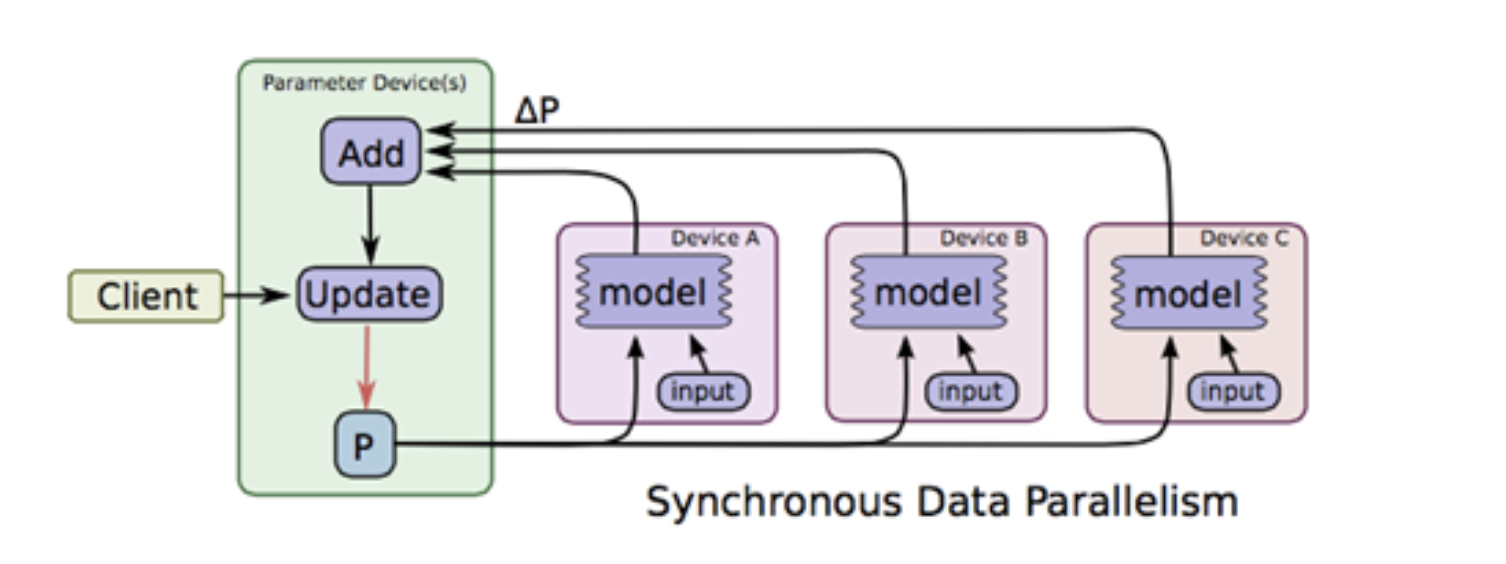
\includegraphics[width=1\textwidth]{fig/Large_Scale_Data_Parallerism.png}
\end{figure}

图片取材于TensorFlow的paper[1.4],图中ABC代表三台不同的机器,上面存储着不同的样本,模型P在各台机器上计算对应的增量,然后在参数存储的机器上进行汇总和更新,这就是数据并行。先忽略synchronous,这是同步机制相关的概念,在第三节会有专门介绍。

\textbf{数据并行概念简单,而且不依赖于具体的模型,因此数据并行机制可以作为框架的一种基础功能,对所有算法都生效}。与之不同的是,模型并行因为参数间存在依赖关系(其实数据并行参数更新也可能会依赖所有的参数,但区别在于往往是依赖于上一个迭代的全量参数。而模型并行往往是同一个迭代内的参数之间有强依赖关系,比如DNN网络的不同层之间的参数依照BP算法形成的先后依赖),无法类比数据并行这样直接将模型参数分片而破坏其依赖关系,所以\textbf{模型并行不仅要对模型分片,同时需要调度器来控制参数间的依赖关系}。而每个模型的依赖关系往往并不同,所以模型并行的调度器因模型而异,较难做到完全通用。关于这个问题,CMU的Erix Xing在[1.5]中有所介绍,感兴趣的可以参考。

模型并行的问题定义可以参考姐夫的[1.6],这篇paper也是tensorflow的前身相关的总结,其中图
\begin{figure}[H]
    \centering
    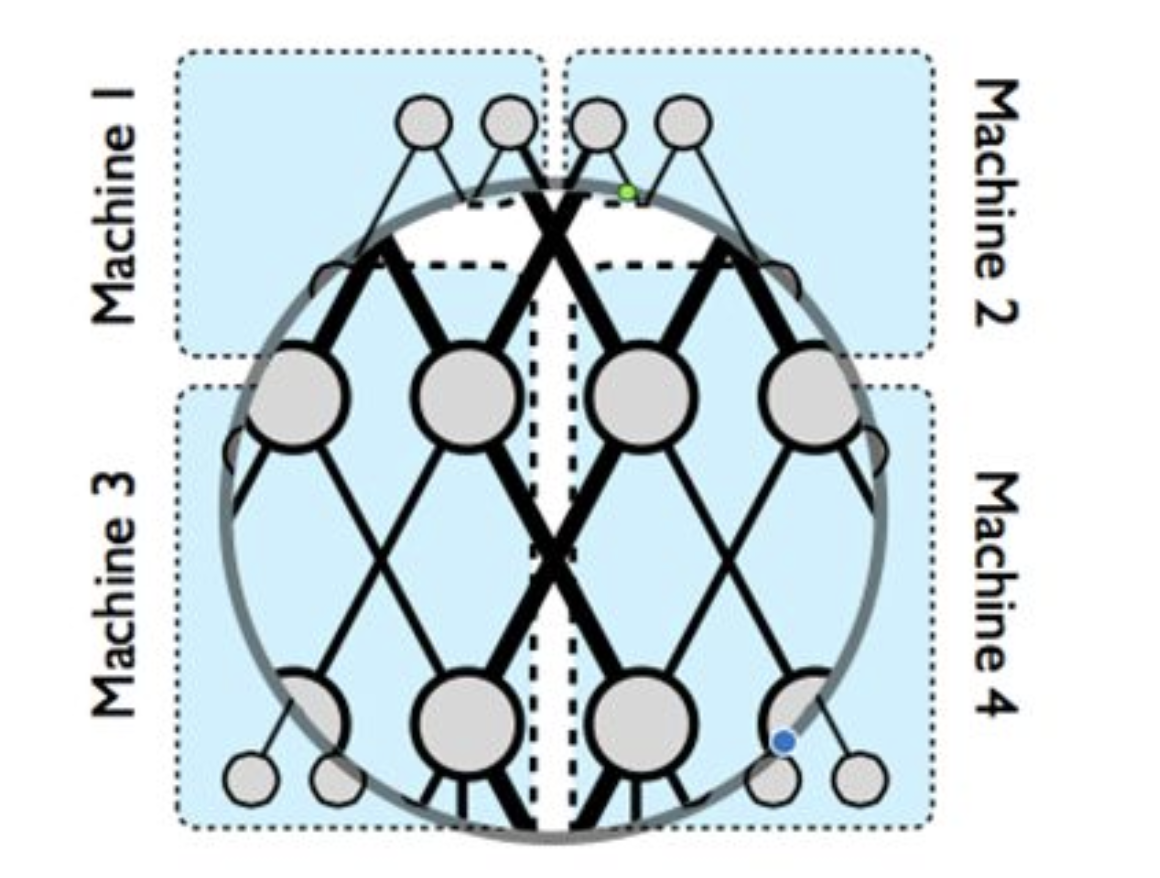
\includegraphics[width=.5\textwidth]{fig/Large_Scale_Model_Parallerism.png}
\end{figure}

解释了模型并行的物理图景,当一个超大神经网络无法存储在一台机器上时,我们可以切割网络存到不同的机器上,但是为了保持不同参数分片之间的依赖,如图中粗黑线的部分,则需要在不同的机器之间进行concurrent控制;同一个机器内部的参数依赖,即途中细黑线部分在机器内即可完成控制。黑线部分如何有效控制呢?如下图所示
\begin{figure}[H]
    \centering
    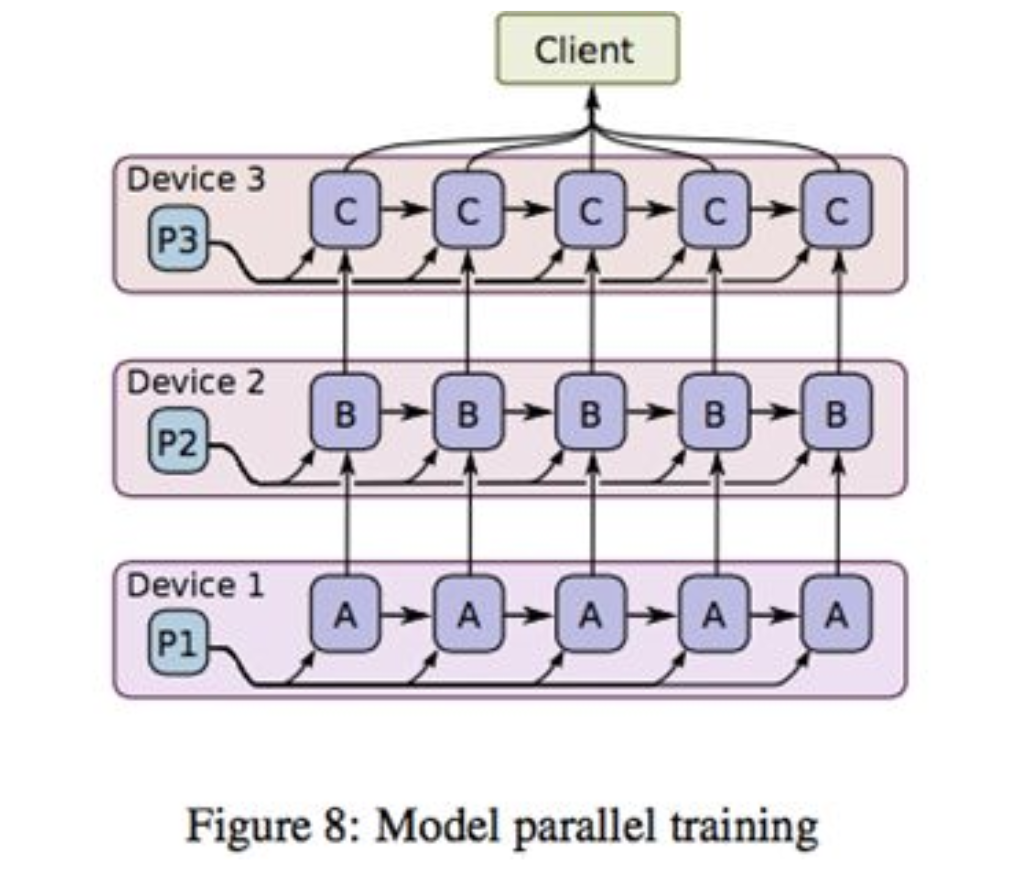
\includegraphics[width=.5\textwidth]{fig/Large_Scale_Model_Parallerism_Training.png}
\end{figure}

在将模型切分到不同机器以后,我们将参数和样本一起在不同机器间流转,途中ABC代表模型的不同部分的参数;假设C依赖B,B依赖A,机器1上得到A的一个迭代后,将A和必要的样本信息一起传到机器2,机器2根据A和样本对P2更新得到,以此类推;当机器2计算B的时候,机器1可以展开A的第二个迭代的计算。了解CPU流水线操作的同学一定感到熟悉,是的,\textbf{模型并行是通过数据流水线来实现并行的}。想想那个盖楼的第二种方案,就能理解模型并行的精髓了。
\begin{figure}[H]
    \centering
    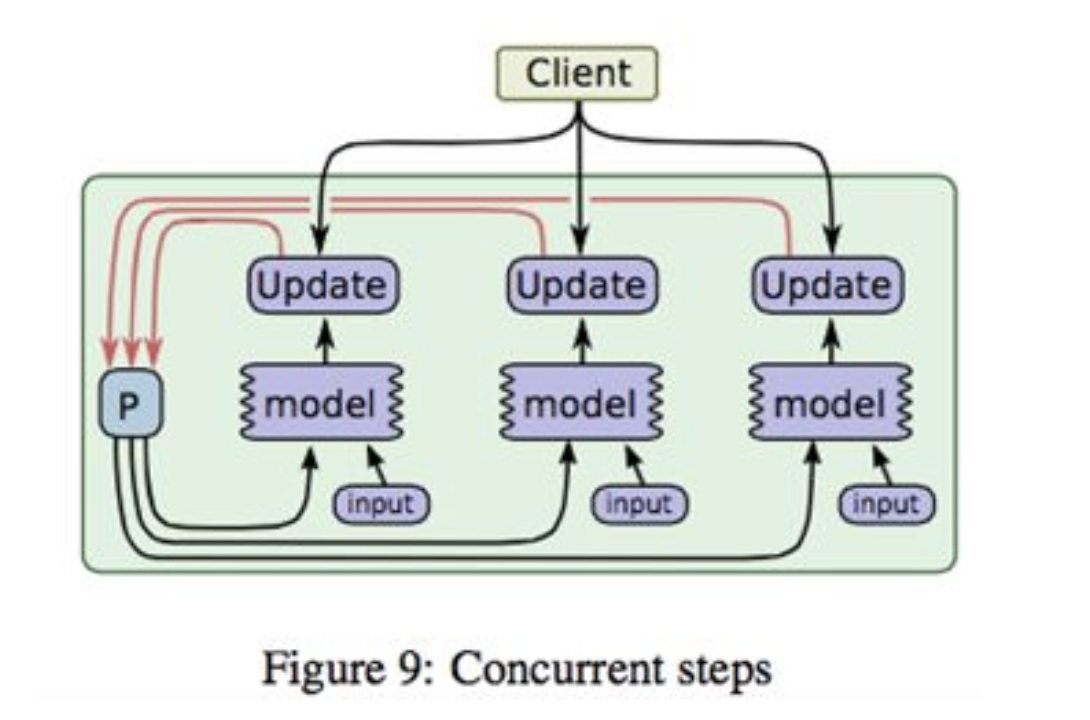
\includegraphics[width=.6\textwidth]{fig/Large_Scale_Concurrent.png}
\end{figure}
上图则是对控制模型参数依赖的调度器的一个示意图,实际框架中一般都会用DAG(有向无环图)调度技术来实现类似功能,未深入研究,以后有机会再补充说明。

理解了数据并行和模型并行对后面参数服务器的理解至关重要,但现在让我先荡开一笔,简单介绍下并行计算框架的一些背景信息。

\section{并行算法演进}
\subsection{MapReduce路线}
从函数式编程中的受到启发,google发布了MapReduce[1.7]的分布式计算方式;通过将任务切分成多个叠加的Map+Reduce任务,来完成复杂的计算任务,示意图如下
\begin{figure}[H]
    \centering
    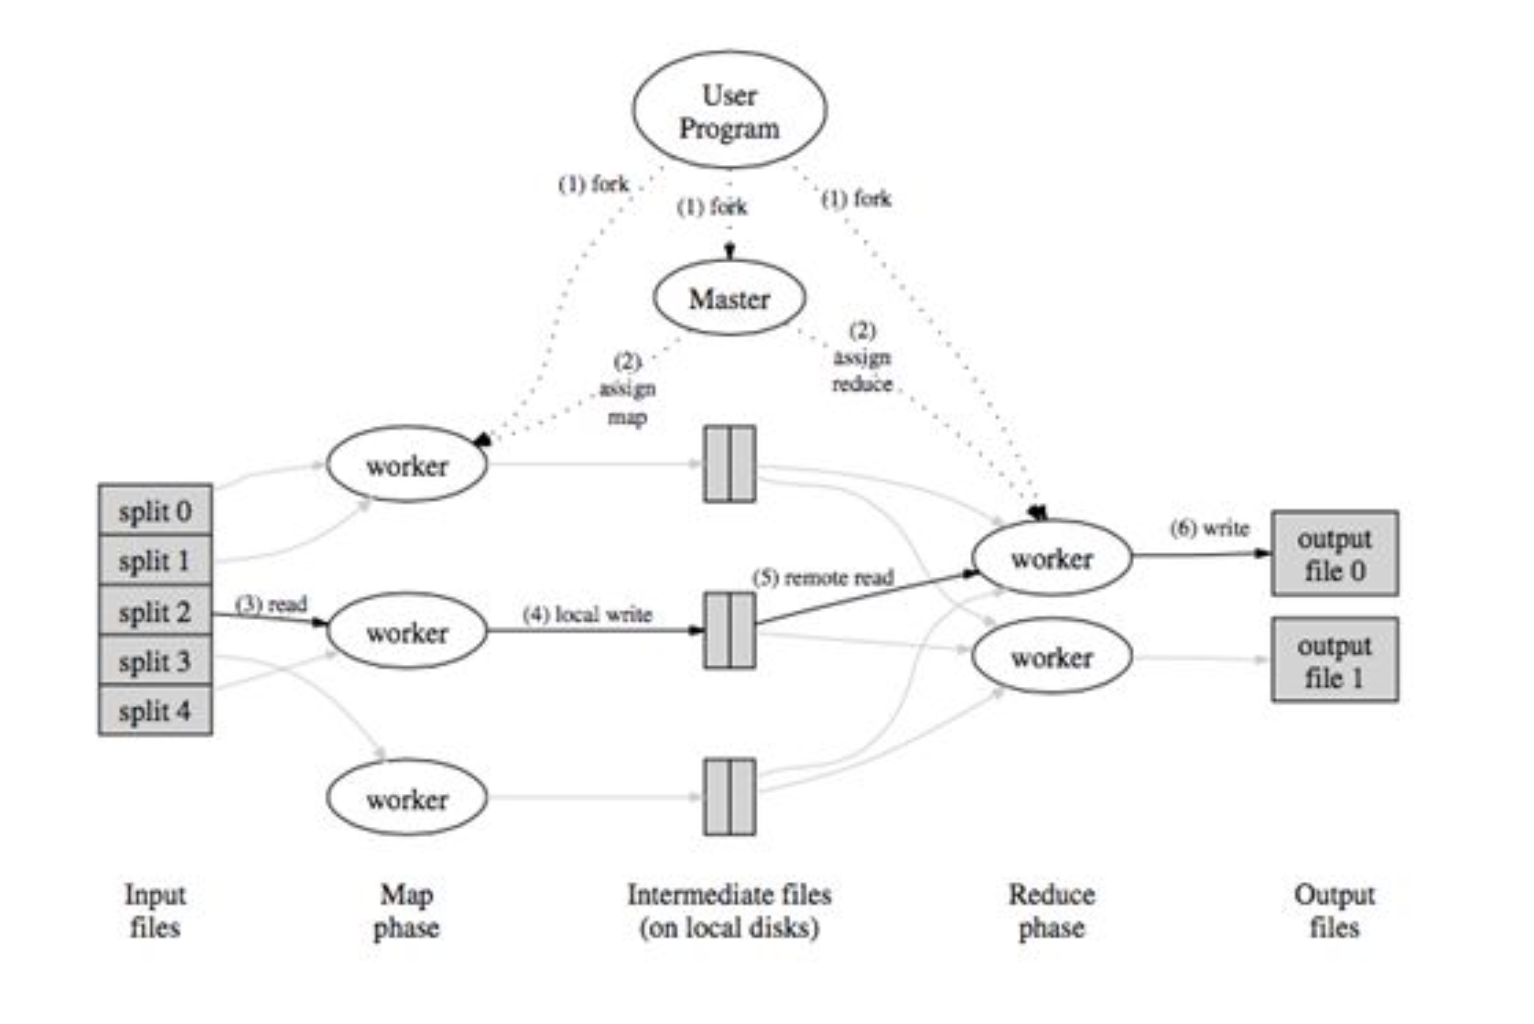
\includegraphics[width=1\textwidth]{fig/Large_Scale_Map_Reduce.png}
\end{figure}

MapReduce的主要问题有两个,\textbf{一是原语的语义过于低级,直接使用其来写复杂算法,开发量比较大;另一个问题是依赖于磁盘进行数据传递,性能跟不上业务需求}。

为了解决MapReduce的两个问题,Matei在[1.8]中提出了一种新的数据结构RDD,并构建了Spark框架。Spark框架在MR语义之上封装了DAG调度器,极大降低了算法使用的门槛。较长时间内spark几乎可以说是大规模机器学习的代表,直至后来沐帅的参数服务器进一步开拓了大规模机器学习的领域以后,spark才暴露出一点点不足。如下图
\begin{figure}[H]
    \centering
    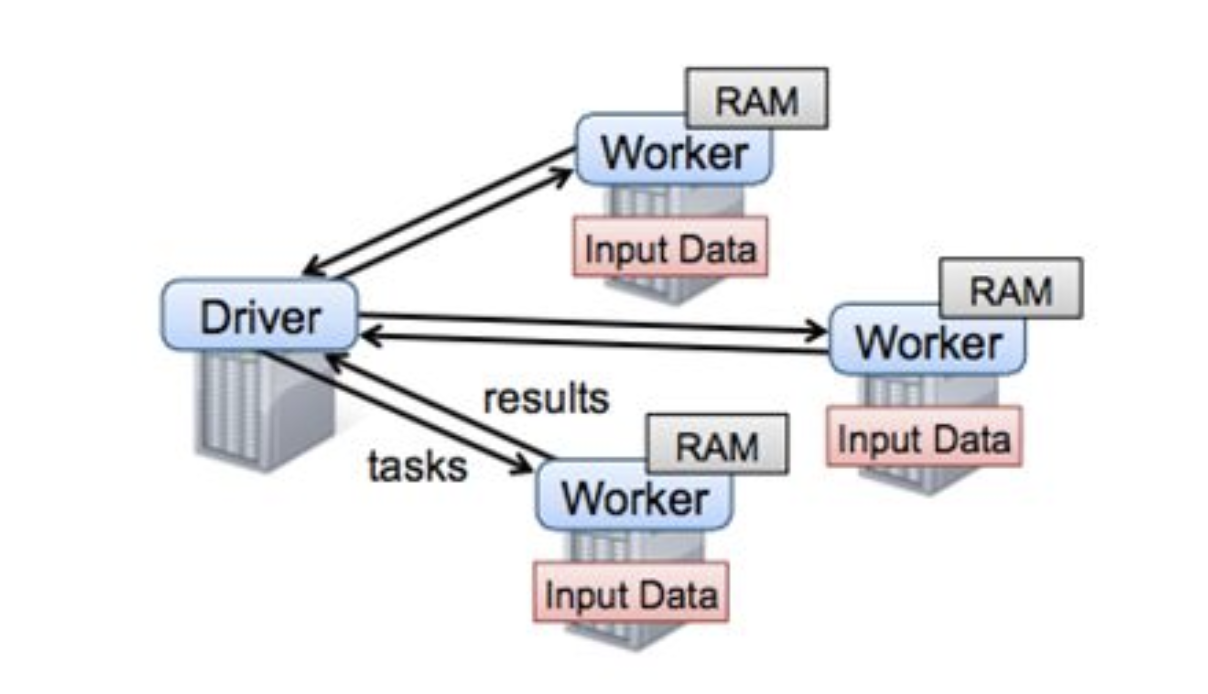
\includegraphics[width=.5\textwidth]{fig/Large_Scale_RDD.png}
\end{figure}

从图中可以看出,\textbf{spark框架以Driver为核心,任务调度和参数汇总都在driver},而driver是单机结构,所以spark的瓶颈非常明显,就在Driver这里。当模型规模大到一台机器存不下的时候,Spark就无法正常运行了。所以从今天的眼光来看,Spark只能称为一个中等规模的机器学习框架。剧透一句,公司开源的Angel通过修改Driver的底层协议将Spark扩展到了一个高一层的境界。后面还会再详细介绍这部分。

MapReduce不仅是一个框架,还是一种思想,google开创性的工作为我们找到了大数据分析的一个可行方向,时至今日,仍不过时。只是逐渐从业务层下沉到底层语义应该处于的框架下层。

\subsection{MPI技术}
沐帅在[1.9]中对MPI的前景做了简要介绍;和Spark不同,MPI是类似socket的一种系统通信API,只是支持了消息广播等功能。因为对MPI研究不深入,这里简单介绍下优点和缺点吧;优点是系统级支持,性能杠杠的;缺点也比较多,一是和MR一样因为原语过于低级,用MPI写算法,往往代码量比较大。另一方面是基于MPI的集群,如果某个任务失败,往往需要重启整个集群,而MPI集群的任务成功率并不高。阿里在[1.10]中给出了下图:
\begin{figure}[H]
    \centering
    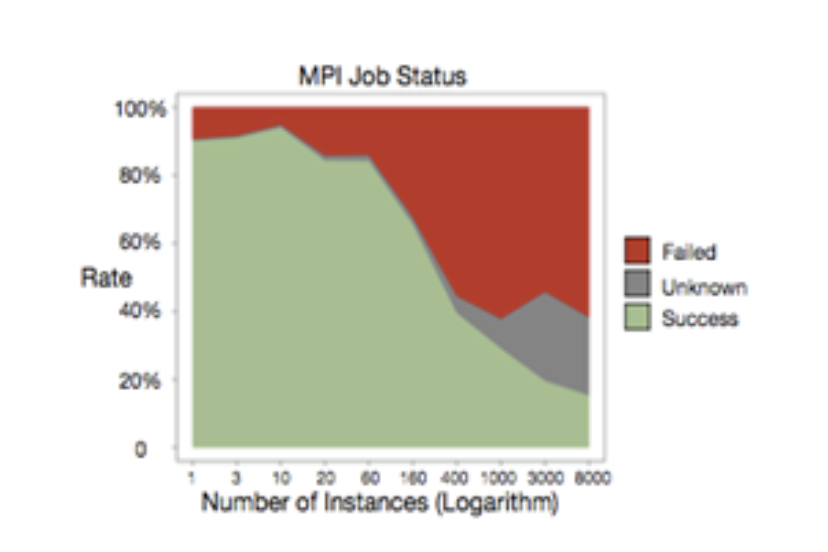
\includegraphics[width=.5\textwidth]{fig/Large_Scale_MPI.png}
\end{figure}
从图中可以看出,MPI作业失败的几率接近五成。MPI也并不是完全没有可取之处,正如沐帅所说,在超算集群上还是有场景的。对于工业届依赖于云计算、依赖于commodity计算机来说,则显得性价比不够高。当然如果在参数服务器的框架下,对单组worker再使用MPI未尝不是个好的尝试,[1.10]的鲲鹏系统正式这么设计的。

\section{参数服务器演进}
\subsection{历史演进}
沐帅在[1.12]中将参数服务器的历史划分为三个阶段,第一代参数服务器萌芽于沐帅的导师Smola的[1.11],如下图所示:
\begin{figure}[H]
    \centering
    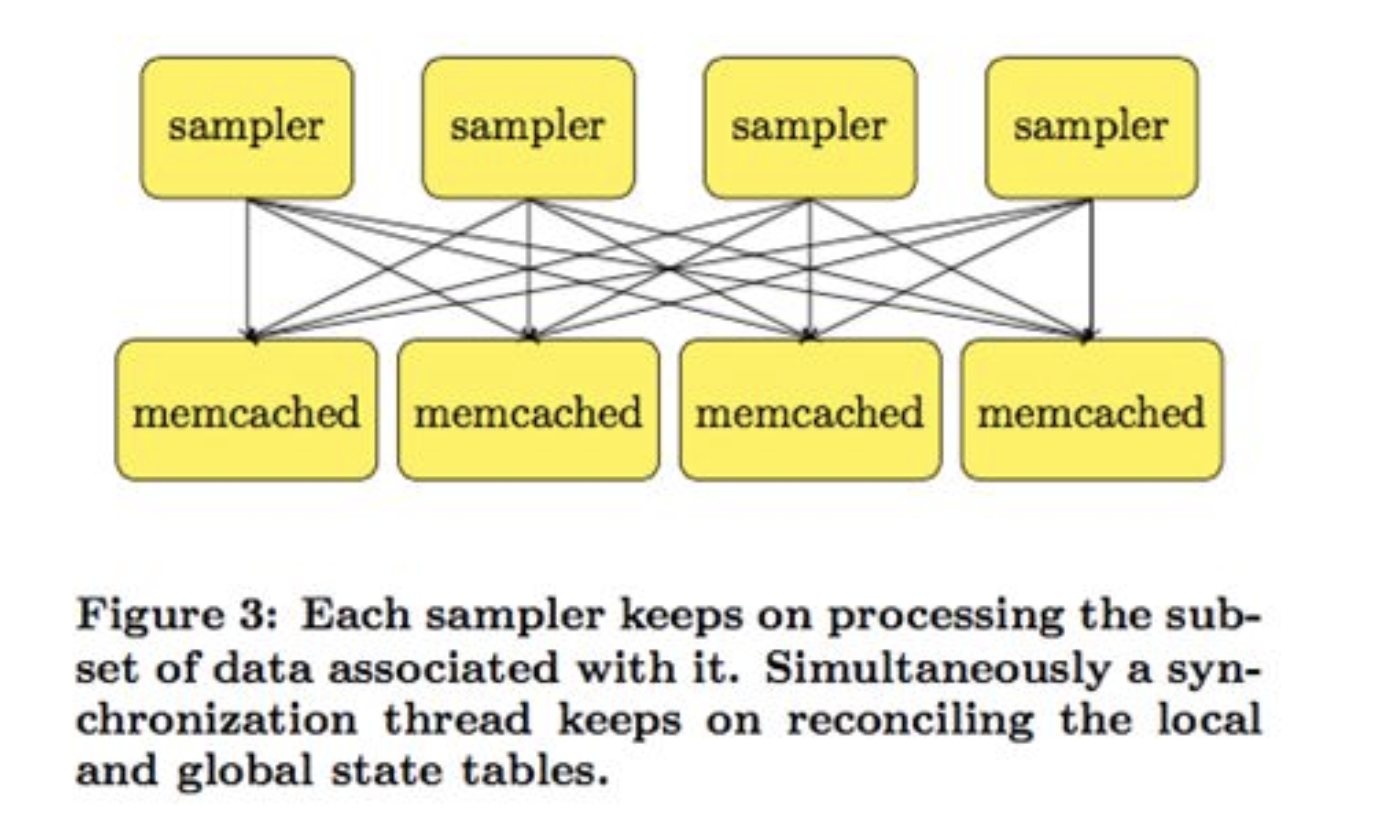
\includegraphics[width=.6\textwidth]{fig/Large_Scale_Parameter_Server_Epoch_1.png}
\end{figure}
这个工作中仅仅引入memcached来存放key-value数据(memcached是一套分布式的高速缓存系统),不同的处理进程并行对其进行处理。[1.13]中也有类似的想法,第二代参数服务器叫application-specific参数服务器,主要针对特定应用而开发,其中最典型的代表应该是tensorflow的前身[1.6]。

第三代参数服务器,也即是通用参数服务器框架是由百度少帅李沐正式提出的,和前两代不同,第三代参数服务器从设计上就是作为一个通用大规模机器学习框架来定位的。要摆脱具体应用、算法的束缚,做一个通用的大规模机器学习框架,首先就要定义好框架的功能;而所谓框架,往往就是把大量重复的、琐碎的、做了一次就不想再来第二次的脏活、累活进行良好而优雅的封装,让使用框架的人可以只关注与自己的核心逻辑。第三代参数服务器要对那些功能进行封装呢?沐帅总结了这几点,我照搬如下:

1). \textbf{高效的网络通信:}因为不管是模型还是样本都十分巨大,因此对网络通信的高效支持以及高配的网络设备都是大规模机器学习系统不可缺少的;


2). \textbf{灵活的一致性模型:}不同的一致性模型其实是在模型收敛速度和集群计算量之间做tradeoff;要理解这个概念需要对模型性能的评价做些分析,暂且留到下节再介绍;

3). \textbf{弹性可扩展:}显而易见;

4). \textbf{容灾容错:}大规模集群协作进行计算任务的时候,出现Straggler或者机器故障是非常常见的事,因此系统设计本身就要考虑到应对;没有故障的时候,也可能因为对任务时效性要求的变化而随时更改集群的机器配置。这也需要框架能在不影响任务的情况下能做到机器的热插拔;

5). \textbf{易用性:}主要针对使用框架进行算法调优的工程师而言,显然,一个难用的框架是没有生命力的。

在正式介绍第三代参数服务器的主要技术之前,先从另一个角度来看下大规模机器学习框架的演进
\begin{figure}[H]
    \centering
    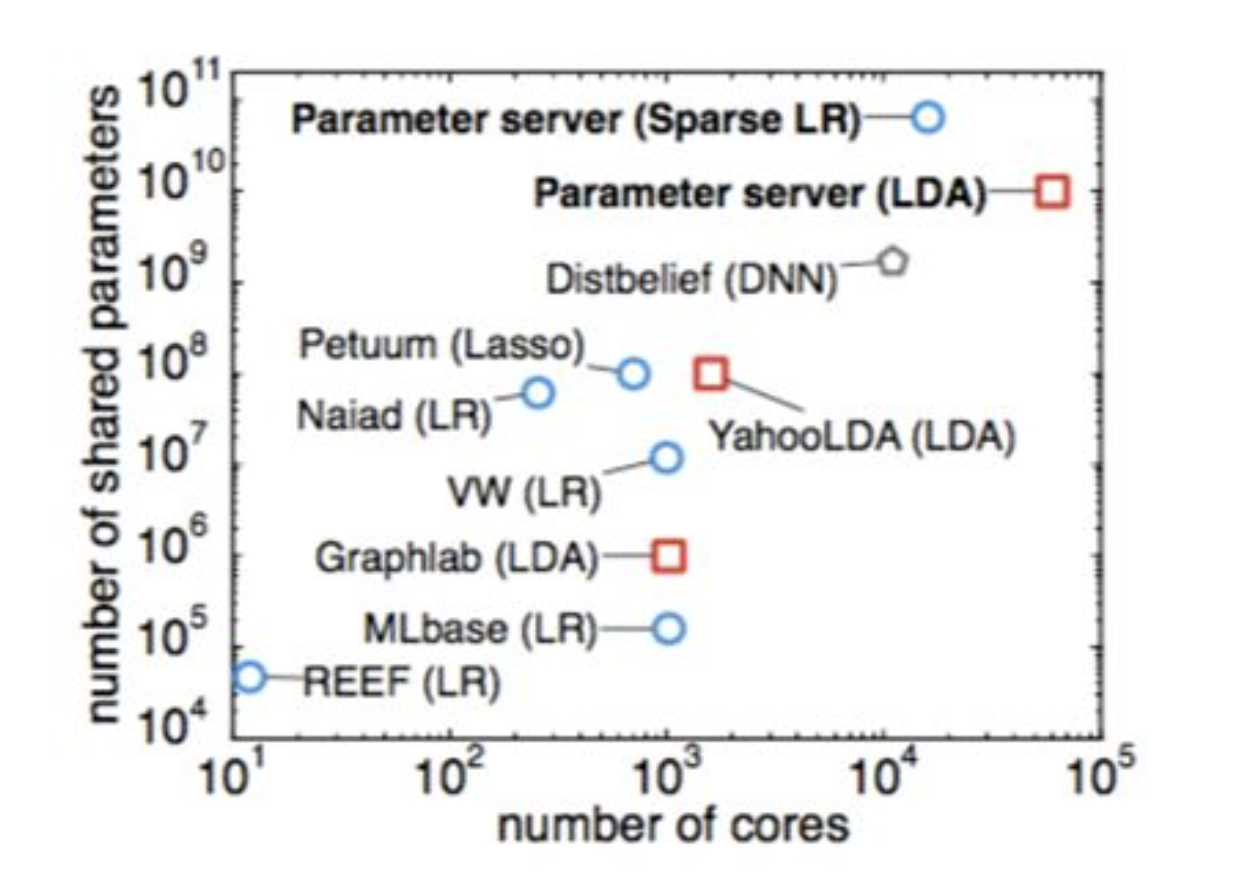
\includegraphics[width=.6\textwidth]{fig/Large_Scale_Framework_Evolution.png}
\end{figure}
这张图可以看出,在参数服务器出来之前,人们已经做了多方面的并行尝试,不过往往只是针对某个特定算法或特定领域,比如YahooLDA是针对LDA算法的。当模型参数突破十亿以后,则可以看出参数服务器一统江湖,再无敌手。

首先我们看看第三代参数服务器的基本架构
\begin{figure}[H]
    \centering
    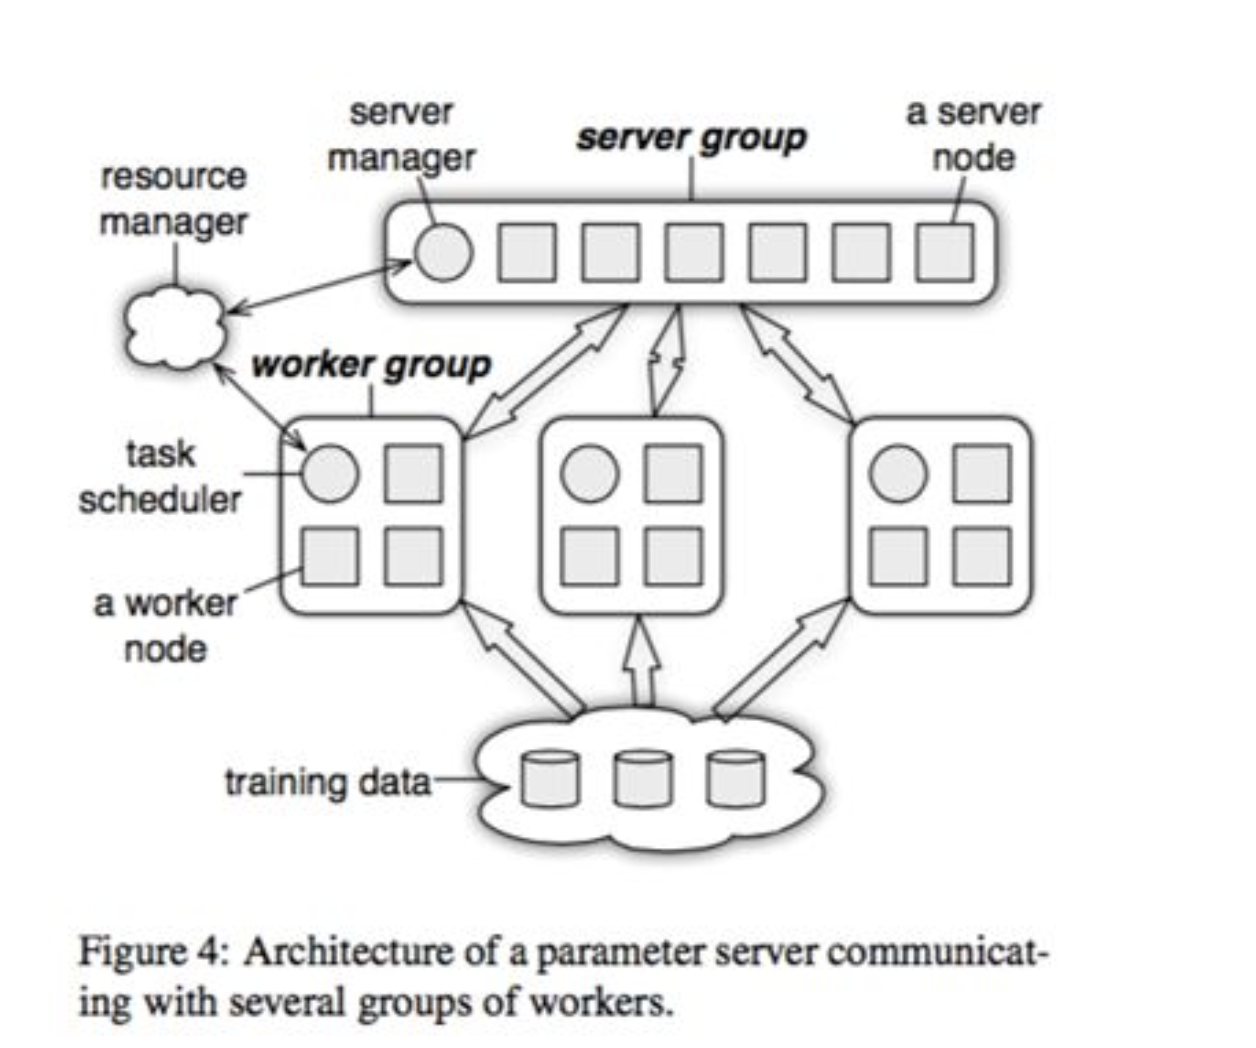
\includegraphics[width=.6\textwidth]{fig/Large_Scale_Parameter_Server_Epoch_3.png}
\end{figure}

上图的resourcemanager可以先放一放,因为实际系统中这部分往往是复用现有的资源管理系统,比如yarn或者mesos;底下的training data毋庸置疑的需要类似GFS的分布式文件系统的支持;剩下的部分就是参数服务器的核心组件了。

图中画了一个server group和三个worker group;实际应用中往往也是类似,server group用一个,而worker group按需配置;server manager是server group中的管理节点,一般不会有什么逻辑,只有当有server node加入或退出的时候,为了维持一致性哈希而做一些调整。

Worker group中的task schedule则是一个简单的任务协调器,一个具体任务运行的时候,task schedule负责通知每个worker加载自己对应的数据,然后去server node上拉取一个要更新的参数分片,用本地数据样本计算参数分片对应的变化量,然后同步给server node;server node在收到本机负责的参数分片对应的所有worker的更新后,对参数分片做一次update。
\begin{figure}[H]
    \centering
    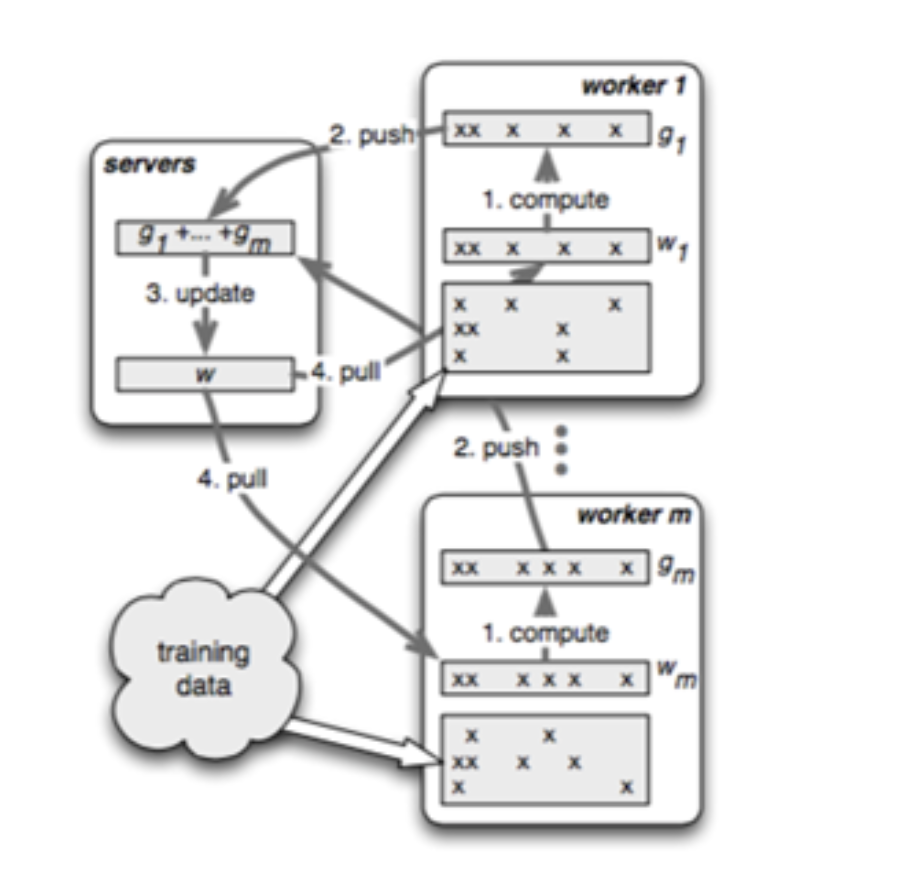
\includegraphics[width=.6\textwidth]{fig/Large_Scale_Parameter_Server_Epoch_3_Worker.png}
\end{figure}
如图所示,不同的worker同时并行运算的时候,可能因为网络、机器配置等外界原因,导致不同的worker的进度是不一样的,如何控制worker的同步机制是一个比较重要的课题。详见下节分解。

\subsection{同步协议}
本节假设读者已经对随机梯度优化算法比较熟悉,如果不熟悉的同学请参考吴恩达经典课程机器学习中对SGD的介绍,或者我之前多次推荐过的书籍《最优化导论》。

我们先看一个单机算法的运行过程,假设一个模型的参数切分成三个分片k1,k2,k3;比如你可以假设是一个逻辑回归算法的权重向量被分成三段。我们将训练样本集合也切分成三个分片s1,s2,s3;在单机运行的情况下,我们假设运行的序列是(k1,s1)、(k2,s1)、(k3、s1)、(k1、s2)、(k2、s2)、(k3、s2)。。。看明白了吗?就是假设先用s1中的样本一次对参数分片k1、k2、k3进行训练,然后换s2;这就是典型的单机运行的情况,而我们知道这样的运行序列最后算法会收敛。

现在我们开始并行化,假设k1、k2、k3分布在三个server node上,s1、s2、s3分布在三个worker上,这时候如果我们还要保持之前的计算顺序,则会变成怎样?work1计算的时候,work2和worker3只能等待,同样worker2计算的时候,worker1和work3都得等待,以此类推;可以看出这样的并行化并没有提升性能;但是也算简单解决了超大规模模型的存储问题。

为了解决性能的问题,业界开始探索这里的一致性模型,最先出来的版本是前面提到的[1.11]中的ASP模式,就是完全不顾worker之间的顺序,每个worker按照自己的节奏走,跑完一个迭代就update,然后继续,这应该是大规模机器学习中的freestyle了,如图所示
\begin{figure}[H]
    \centering
    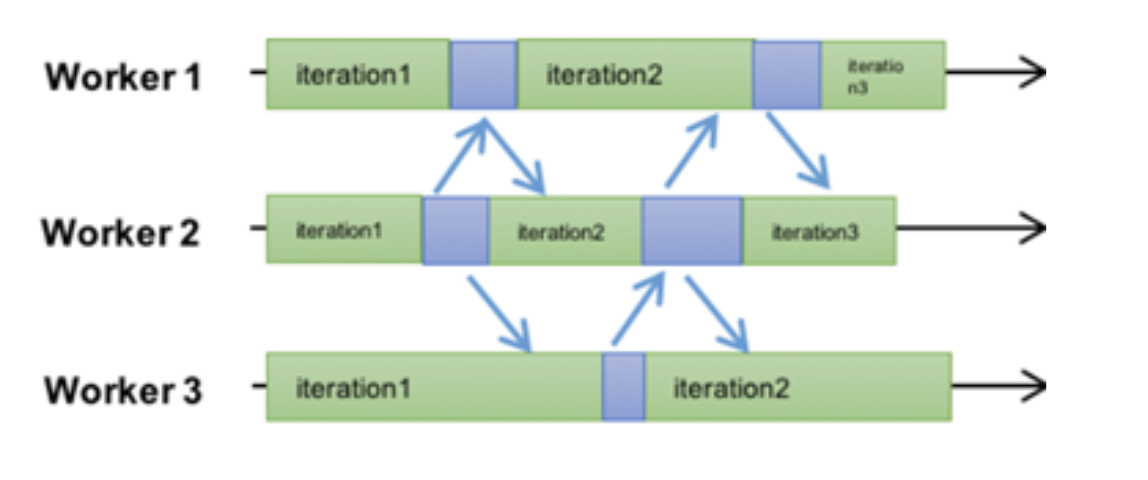
\includegraphics[width=1\textwidth]{fig/Large_Scale_Synchronize_ASP.png}
\end{figure}

在ASP之后提出了另一种相对极端的同步协议BSP,spark用的就是这种方式,如图所示
\begin{figure}[H]
    \centering
    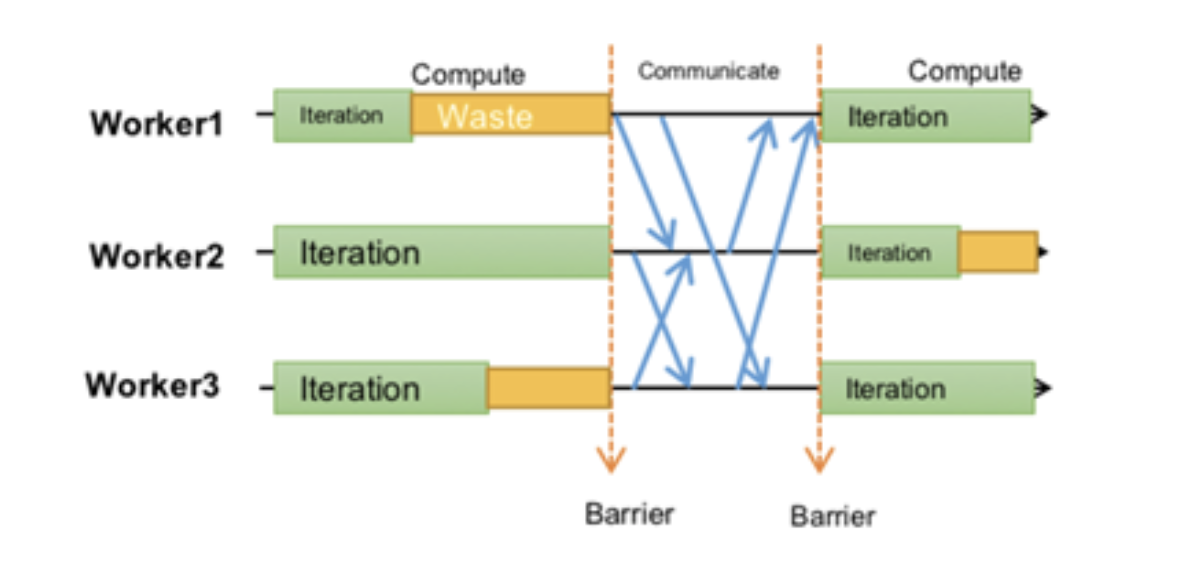
\includegraphics[width=1\textwidth]{fig/Large_Scale_Synchronize_BSP.png}
\end{figure}
每个worker都必须在同一个迭代运行,只有一个迭代任务所有的worker都完成了,才会进行一次worker和server之间的同步和分片更新。这个算法和严格一直的算法非常类似,区别仅仅在于单机版本的batch size在BSP的时候变成了有所有worker的单个batch size求和得到的总的batch size替换。毫无疑问,\textbf{BSP的模式和单机串行因为仅仅是batch size的区别,所以在模型收敛性上是完全一样的}。同时,因为每个worker在一个周期内是可以并行计算的,所以有了一定的并行能力。

以此协议为基础的spark在很长时间内成为机器学习领域实际的霸主,不是没有理由的。此种协议的缺陷之处在于,整个worker group的性能由其中最慢的worker决定;这个worker一般称为straggler。读过GFS文章的同学应该都知道straggler的存在是非常普遍的现象。

能否将ASP和BSP做一下折中呢?答案当然是可以的,这就是目前我认为最好的同步协议SSP;SSP的思路其实很简单,既然ASP是允许不同worker之间的迭代次数间隔任意大,而BSP则只允许为0,那我是否可以取一个常数s?如图所示
\begin{figure}[H]
    \centering
    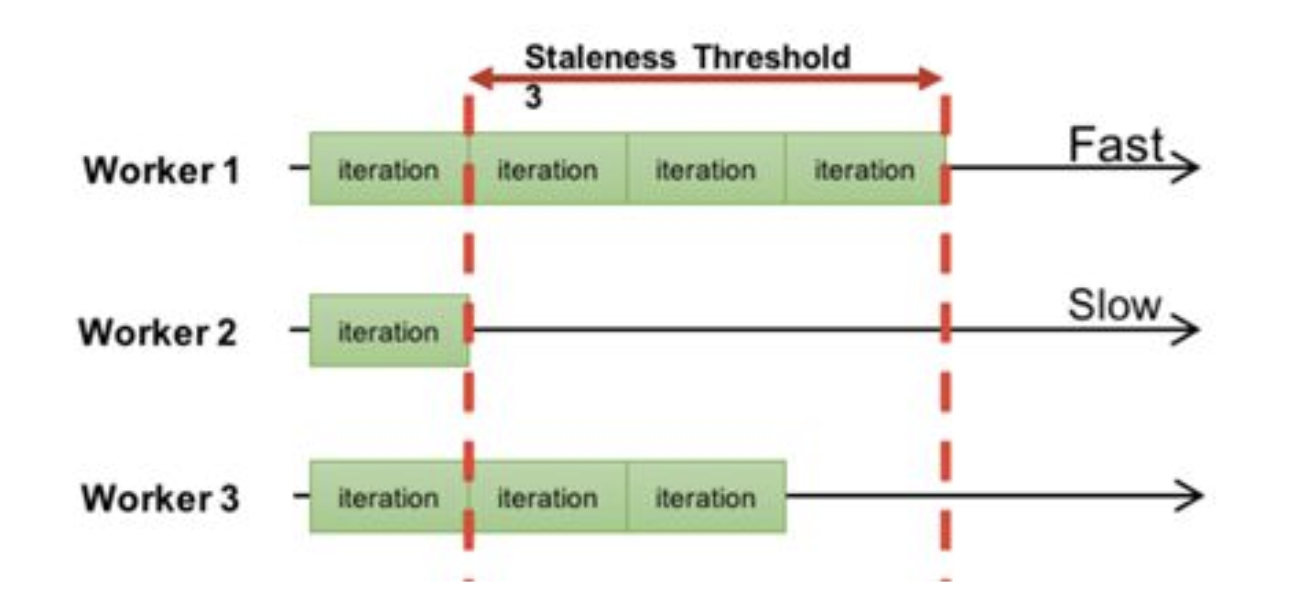
\includegraphics[width=1\textwidth]{fig/Large_Scale_Synchronize_SSP.png}
\end{figure}
不同的worker之间允许有迭代的间隔,但这个间隔数不允许超出一个指定的数值s,图中s=3.

SSP协议的详细介绍参见[1.14],CMU的大拿Eric Xing在其中详细介绍了SSP的定义,以及其收敛性的保证。理论推导证明常数s不等于无穷大的情况下,算法一定可以在若干次迭代以后进入收敛状态。其实在Eric提出理论证明之前,工业界已经这么尝试过了:)

顺便提一句,考察分布式算法的性能,一般会分为statistical performance和hard performance来看。前者指不同的同步协议导致算法收敛需要的迭代次数的多少,后者是单次迭代所对应的耗时。两者的关系和precision/recall关系类似,就不赘述了。有了SSP,BSP就可以通过指定s=0而得到。而ASP同样可以通过制定$s=\infty$来达到。

\subsection{核心技术}
除了参数服务器的架构、同步协议之外,本节再对其他技术做一个简要的介绍,详细的了解请直接阅读沐帅的博士论文和相关发表的论文。

热备、冷备技术:为了防止server node挂掉,导致任务中断,可以采用两个技术,一个是对参数分片进行热备,每个分片存储在三个不同的server node中,以master-slave的形式存活。如果master挂掉,可以快速从slave获取并重启相关task。

除了热备,还可以定时写入checkpoint文件到分布式文件系统来对参数分片及其状态进行备份。进一步保证其安全性。

Server node管理:可以使用一致性哈希技术来解决server node的加入和退出问题,如图所示
\begin{figure}[H]
    \centering
    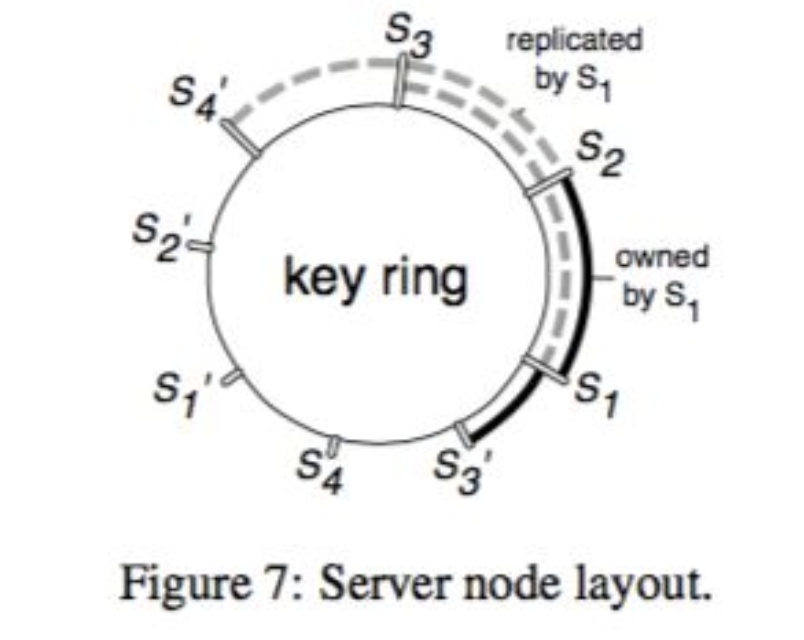
\includegraphics[width=.5\textwidth]{fig/Large_Scale_Server_Node_Layout.png}
\end{figure}
当有server node加入或退出的时候,server manager负责对参数进行重新分片或者合并。注意在对参数进行分片管理的情况下,一个分片只需要一把锁,这大大提升了系统的性能,也是参数服务器可以实用的一个关键点。

\section{大规模机器学习的四重境界}
到这里可以回到我们的标题了,大规模机器学习的四重境界到底是什么呢?这四重境界的划分是作者个人阅读总结的一种想法,并不是业界标准,仅供大家参考。

\subsection{境界1:参数可单机存储和更新}
此种境界较为简单,但仍可以使用参数服务器,通过数据并行来加速模型的训练。

\subsection{境界2:参数不可单机存储,可以单机更新}
此种情况对应的是一些简单模型,比如sparse logistic regression;当feature的数量突破百亿的时候,LR的权重参数不太可能在一台机器上完全存下,此时必须使用参数服务器架构对模型参数进行分片。但是注意一点,SGD的更新公式 $w' = w -\alpha$,其中可以分开到单个维度进行计算,但是单个维度的$w_i = f(w)x_i$

这里的$f(w)$表示是全部参数$w$的一个函数,具体推倒比较简单,这里篇幅所限就不赘述了。只是想说明worker在计算梯度的时候可能需要使用到上一轮迭代的所有参数。而我们之所以对参数进行分片就是因为我们无法将所有参数存放到一台机器,现在单个worker有需要使用所有的参数才能计算某个参数分片的梯度,这不是矛盾吗?可能吗?

答案是可能的,因为单个样本的feature具有很高的稀疏性(sparseness)。例如一个百亿feature的模型,单个训练样本往往只在其中很小一部分feature上有取值,其他都为0(假设feature取值都已经离散化了)。因此计算$f(w)$的时候可以只拉取不为0的feature对应的那部分$w$即可。有文章统计一般这个级别的系统,稀疏性往往在0.1\%(or 0.01\%,记得不是很准,大致这样)以下。这样的稀疏性,可以让单机没有任何阻碍的计算$f(w)$。

目前公司开源的angel和AILab正在做的系统都处于这个境界。而原生spark还没有达到这个境界,只能在中小规模的圈子里厮混。Angel改造的基于Angel的Spark则达到了这个境界。

\subsection{境界3:参数不可单机存储,不可单机更新,但无需模型并行}
境界3顺延境界2二来,当百亿级feature且feature比较稠密的时候,就需要计算框架进入到这层境界了,此时单个worker的能力有限,无法完整加载一个样本,也无法完整计算$f(w)$。怎么办呢?其实很简单,学过线性代数的都知道,矩阵可以分块。向量是最简单的矩阵,自然可以切成一段一段的来计算。只是调度器需要支持算符分段而已了。

\subsection{境界4:参数不可单机存储,不可单机更新,需要模型并行}
进入到这个层次的计算框架,可以算是世界一流了。可以处理超大规模的神经网络。这也是最典型的应用场景。此时不仅模型的参数不能单机存储,而且同一个迭代内,模型参数之间还有强的依赖关系,可以参见姐夫对distbelief的介绍里的模型切分。

此时首先需要增加一个coordinator组件来进行模型并行的concurrent控制。同时参数服务器框架需要支持namespace切分,coordinator将依赖关系通过namespace来进行表示。

一般参数间的依赖关系因模型而已,所以较难抽象出通用的coordinator来,而必须以某种形式通过脚本parser来生产整个计算任务的DAG图,然后通过DAG调度器来完成。对这个问题的介绍可以参考Erix Xing的分享[1.5]。

\subsection{Tensorflow}
目前业界比较知名的深度学习框架有Caffee、MXNet、Torch、Keras、Theano等,但目前最炙手可热的应该是google发布的Tensorflow。这里单独拿出来稍微分解下。

前面不少图片引自此文,从TF的论文来看,TF框架本身是支持模型并行和数据并行的,内置了一个参数服务器模块,但从开源版本所曝光的API来看,TF无法用来10B级别feature的稀疏LR模型。原因是已经曝光的API只支持在神经网络的不同层和层间进行参数切分,而超大规模LR可以看做一个神经单元,TF不支持单个神经单元参数切分到多个参数服务器node上。

当然,以google的实力,绝对是可以做到第四重境界的,之所以没有曝光,可能是基于其他商业目的的考量,比如使用他们的云计算服务。

综上,个人认为如果能做到第四重境界,目前可以说的上是世界一流的大规模机器学习框架。仅从沐帅的ppt里看他曾经达到过,google内部应该也是没有问题的。第三重境界应该是国内一流,第二充应该是国内前列吧。

\section{其他}
\subsection{资源管理}
本文没有涉及到的部分是资源管理,大规模机器学习框架部署的集群往往资源消耗也比较大,需要专门的资源管理工具来维护。这方面yarn和mesos都是佼佼者,细节这里也就不介绍了。

\subsection{设备}
除了资源管理工具,本身部署大规模机器学习集群本身对硬件也还是有些要求的,虽然理论上来说,所有commodity机器都可以用来搭建这类集群,但是考虑到性能,我们建议尽量用高内存的机器+万兆及以上的网卡。没有超快速的网卡,玩参数传递和样本加载估计会比较苦逼。

\section{引用文献}
1.1. Wide\& Deep Learning for Recommender Systems

1.2. Deep Neural Networks for YouTube Recommendations

1.3. \url{https://www.zhihu.com/question/53851014}

1.4. TensorFlow:Large-Scale Machine Learning on Heterogeneous Distributed Systems

1.5. \url{http://www.jianshu.com/p/00736aa21dc8}

1.6. Large Scale Distributed Deep Networks

1.7. MapReduce: Simplified Data Processing on Large
Clusters

1.8. Resilient Distributed Datasets: A Fault-Tolerant Abstraction for In-Memory Cluster Computing

1.9. \url{https://www.zhihu.com/question/55119470}

1.10. KunPeng:Parameter Server based Distributed Learning Systems and Its Applications in
Alibaba and Ant Financial

1.11. An Architecture for Parallel Topic Models

1.12. Scaling Distributed Machine Learning with the Parameter Server

1.13. Piccolo:Building fast, distributed pro- grams with partitioned tables 


1.14. More Effective Distributed ML via a Stale Synchronous Parallel Parameter Server

1.15. Angel-A Flexible and Powerful Parameter Server;黄明ppt

\part{深度学习加速:算法、编译器、体系结构与硬件设计\cite{Deep_Learning_Speed_Up}}
\setcounter{section}{0}
\section{算法顶层}
算法顶层在深度学习加速的工作也囊括了很多方面,例如:更好的分布式训练调度(大规模分布式机器学习系统),更好的优化算法,更简单高效的神经网络结构,更自动化的网络搜索机制(神经网络架构搜索NAS), 更有效的网络参数量化剪枝算法、卷积运算的优化等等。

\subsection{大规模分布式机器学习}
这方面主要是分布式系统的一些设计。现在的网络模型越来越大,为了达到好的拟合效果,许多公司需要用极大的数据量喂给模型训练,这些数据往往单机都塞不下,而要一个batch一个batch慢慢给可能要训练到猴年马月,因此才需要大规模分布式机器学习系统。

下面内容先概括:
\begin{itemize}
\setlength{\itemsep}{0pt}
\setlength{\parsep}{0pt}
\setlength{\parskip}{0pt}
    \item \textbf{并行方式有数据并行和模型并行}
    \item \textbf{调度方式有集中式(参数服务器)和去中心化调度(RingAllReduce)}
    \item \textbf{参数更新方式有同步和异步两种,从另外角度分的话有基于参数的,有基于梯度方式的}
\end{itemize}

分布式机器学习系统的并行加速本质上是就是DLP的多机延伸,具体来说其并行的方式分为两种:
\subsubsection{数据并行}
顾名思义就是每台机器都有模型的副本,但是将数据的不同部分分别喂给各个模型(各个机器), 最后的结果以某种方式进行合并(可能是直接参数融合,也可能是传递梯度数据进行融合)。数据并行是最常见也是最直观可以理解的。

\subsubsection{模型并行}
模型并行的话,就是模型本身太大了,因此需要将模型各个部分分散在各个机器间,这种情况在更新参数时需要层间跨机器通信。


\subsubsection{两者结合}
当然实际上还会有数据并行和模型并行的结合,可以从这个角度理解: 模型各个部分分散在单机的多个GPU中(模型并行),同时模型在多个机器都有副本,数据各个部分分别喂给各个机器并行训练(数据并行)。

上面介绍的是并行的方式,那么在实际分布式训练中是怎么进行训练的调度呢?调度方式主要分为集中式调度 和 去中心化调度,前者代表有Parameter Server方式,后者代表有Ring Allreduce方式。

\subsubsection{Parameter Server}
参数服务器是一种集中式的架构,有专门的机器用于存放全局参数,其他的worker用于训练!那么怎么更新呢?

\textbf{一种方法是参数平均,这是一种同步方式}。这种方式下,参数服务器每次将全局参数分配到各个worker,worker们每次迭代更新了参数后再汇集到参数服务器求平均得到这一轮的结果,之后再重复上述步骤直到收敛,是不是很简单!然而实际在工程上要考虑更多!例如,由于参数服务器要等待所有worker的参数到来后才可以操作(同步方式),那么如果有worker发生故障呢? 如果worker每一次迭代就发参数给参数服务器,那么通信可能会成为瓶颈,而我们知道,计算比重 要大于传输比重,才有收益,所以可能需要考虑在worker那边多做几轮迭代后再给参数服务器更新,减少通信开销。诸如此类的衡量还有很多。

另一种就是基于梯度的方式,worker不是发送本地更新后的参数给参数服务器,而是发送梯度数据,参数服务器汇总的是梯度,然后在那边统一进行梯度更新。这也是一种同步更新的方式!两种方式似乎大同小异,但是由于\textbf{梯度的稀疏特性},在通信前可以利用压缩算法来减少传输开销。

参数平均和基于梯度的方式本质上都是同步更新方式,有同步就有异步方式(基于梯度的方法本身可以做成异步更新的方式)。异步是说参数服务器不再等待最后一个worker才开始操作,而是有worker的参数到了,我这边就开算,不进行等待。那么两种更新方式的区别如下:

\begin{itemize}
\setlength{\itemsep}{0pt}
\setlength{\parsep}{0pt}
\setlength{\parskip}{0pt}
    \item 同步方式: 有较大通信开销和同步等待开销,但是优点是收敛过程比较稳定。
    \item 异步方式: 速度快,高吞吐,等待时间少。但是噪声更大,有参数过期问题,所以收敛过程没有前者稳定。
\end{itemize}

\subsubsection{Ring AllReduce}
这种调度方式是与Parameter Server相反的方式,体现了设备去中心化思想。集中式调度容易管理,但是随着worker数目增加,master的负担越来越大,加速比也急剧恶化。

而 Ring AllReduce可以将参数通信分散到各个GPU,经过一循环的数据传递和计算后,得到正确结果。通过Ring AllReduce这种比较巧妙的方式,每个设备的负载更加均衡,基本上可以实现当GPU并行卡数的增加,实现计算性能的线性增长。具体的scatter和reduce流程可以参考这里,一些相关的分布式训练库: horovod baidu-allreduce

\subsection{优化算法}
深度学习的优化算法我觉得也可以算入深度学习加速的范畴,因为各式各样的优化算法(SGD,Adagrad,Adadelta,RMSprop,Momentum,Adam,Adamax,Nadam)的目标都是使得梯度下降搜索的时候可以更加趋近全局最优,使得收敛的速度更快,从而加速训练进度。当然,优化算法在分布式机器学习系统上需要实现其相应的分布式的版本,各类优化算法在分布式系统的参数更新方式上可以玩出很多花来。

\subsection{(轻量级)高效的神经网络结构}
由于神经网络对于噪声不敏感,所以许多早期经典模型的参数其实是存在很大冗余度的,这样的模型很难部署在存储有限的边缘设备,因此学术界开始追求一些轻量级的网络设计(这代表着更少的参数,更少的乘法操作,更快的速度):

\begin{itemize}
\setlength{\itemsep}{0pt}
\setlength{\parsep}{0pt}
\setlength{\parskip}{0pt}
    \item 减小卷积核大小:主要的做法包括使用更小的3x3卷积(加深网络来弥补感受野变小);将大卷积核分解成一系列小的卷积核的操作组合。
    
    \item 减少通道数:第一种方式:1x1卷积的应用。在大卷积核前应用1X1卷积,可以灵活地缩减feature map通道数(同时1X1卷积也是一种融合通道信息的方式),最终达到减少参数量和乘法操作次数的效果;第二种方式:group convolution,将feature map的通道进行分组,每个filter对各个分组进行操作即可。第三种方式:depthwise convolution,是组卷积的极端情况,每一个组只有一个通道,这样filters参数量进一步下降。如果只采用分组卷积操作,相比传统卷积方式,不同组的feature map信息无法交互,因此可以在组卷积之后在feature map间进行Shuffle Operation来加强通道间信息融合。或者更巧妙的是像Pointwise convolution那样将原本卷积操作分解成两步,先进行 depthwise convolution,之后得到的多个通道的feature map再用一个1X1卷积进行通道信息融合,拆解成这样两步,卷积参数也减少了。
    \item 减少filter数目:直接减少的filter数目虽然可以减少参数,但是导致每层产生的feature map数目减少,网络的表达能力也会下降不少。一个方法是像DenseNet那样,一方面减少每层filter数目,同时在每层输入前充分重用之前每一层输出的feature map。

    \item 池化操作:池化操作是操作卷积神经网络的标准操作,池化层没有参数,同时又可以灵活缩减上一级的feature map大小,从而减少下一级卷积的乘法操作。
\end{itemize}

\subsection{神经网络架构搜索}
1.3节所介绍的那些高效的神经网络结构本质上是人工精心(费力)设计的结构,而神经网络架构搜索NAS则是将神经网络设计探索这个过程自动化。

NAS主要包括三个主要的components:
\begin{itemize}
\setlength{\itemsep}{0pt}
\setlength{\parsep}{0pt}
\setlength{\parskip}{0pt}
    \item 搜索空间:搜索空间的每个样本就是一种神经网络设计架构
    \item 优化算法:如何进行采样得到一种网络设计
    \item 性能评价:用什么指标评价采样出来的网络设计,评价的结果反过来指导优化算法的采样。通常的指标是DNN的accuracy和所需的搜索时间
\end{itemize}

优化总搜索时间可以从缩小搜索空间、提升优化算法和简化性能评价指标三部分入手:
\begin{itemize}
\setlength{\itemsep}{0pt}
\setlength{\parsep}{0pt}
\setlength{\parskip}{0pt}
    \item 缩小搜索空间:可以通过增加一些搜索约束来减少探索空间,例如 权衡架构的宽度;放低所要达到的性能目标;结合domain knowledge,通过现有的人工设计经验来缩小探索范围;
    \item 提升优化算法:关于如何用一种比较好的启发算法从搜索空间采样出网络设计,NAS + 以前优化领域那一系列智能算法又可以玩出各式花样来,遗传算法、模拟退火、粒子群、蚂蚁算法...等等都有相关的结合工作;
    \item 简化性能评价:先在小型轻量级的数据集训练和快速验证,观察验证集精度曲线决定是否早期停止等等,这些经常使用的训练技巧在NAS上也同样适用;
\end{itemize}

\subsection{网络量化剪枝}
\subsubsection{什么是量化}
最简单的理解方式就是:统计网络权重和激活值的取值范围,找到最大值最小值后进行min-max映射把所有的权重和激活映射到到 INT8 整型范围(-127~128)。

\subsubsection{量化为什么有效}
首先量化会损失精度,这相当于给网络引入了噪声,但是神经网络一般对噪声是不太敏感的,只要控制好量化的程度,对高级任务精度影响可以做到很小。

其次,传统的卷积操作都是使用FP32浮点,浮点运算时需要很多时间周期来完成,但是如果我们将权重参数和激活在输入各个层之前量化到INT8,位数少了乘法操作少了,而且此时做的卷积操作都是整型的乘加运算,比浮点快很多,运算结束后再将结果乘上scale\_factor变回FP32,这整个过程就比传统卷积方式快很多。

提前从体系结构的考量角度思考量化带来的另一个好处是节能和芯片面积,怎么理解呢?每个数使用了更少的位数,做运算时需要搬运的数据量少了,减少了访存开销(节能),同时所需的乘法器数目也减少(减少芯片面积)。


\subsubsection{量化的一些其它考量}
上面举的例子都是INT8量化,实际上要根据设备的支持情况以及应用的性能要求选择INT32、INT16、 INT8量化。单纯使用min-max映射可以将分布均匀的浮点数映射到INT8空间,但是如果权重和激活比较多地集中在0.0以上,只有小部分落在负数,那么此时min-max映射后许多数也会集中在INT8某个小范围,那么INT8宝贵的动态范围就被浪费了,因此我们需要选择一个合适的阈值对激活和权重的范围进行裁剪,NIVDIA在实际操作中是根据KL散度来选择出这个裁剪阈值,具体细节参考 章小龙:Int8量化-介绍(一)\url{https://zhuanlan.zhihu.com/p/58182172}

\subsubsection{权重剪枝}
神经网络的权重剪枝就是把网络趋近于0的权重直接裁剪成0,以达到稀疏性。权重剪枝,可以作为量化模型后进一步的优化,有了稀疏性,通过压缩后可以进一步减少参数存储量;有了稀疏性,运算时如果跳过权重为0的计算,又可以减少功耗。TensorFlow Lite框架对模型的移动端部署的核心优化就是量化和权重剪枝。

稀疏模型的优势在于易于可压缩,在推理过程中跳过权重为0的计算。剪枝通过压缩模型来实现。在牺牲微小精度的前提下,我们的模型有6倍的性能提升。剪枝这项技术,也在实际应用到语音应用中,如语音识别、文本转语音以及横跨各种视觉与翻译的模型中。

权重剪枝主要有两种方式:
\begin{itemize}
\setlength{\itemsep}{0pt}
\setlength{\parsep}{0pt}
\setlength{\parskip}{0pt}
    \item 后剪枝:拿到一个模型直接对权重进行剪枝,不需要其他条件;
    \item 训练时剪枝:训练迭代时边剪枝,使网络在训练过程中权重逐渐趋于0,但是由于训练时权重动态调整,使得剪枝操作对网络精度的影响可以减少,所以训练时剪枝比后剪枝更加稳定;
\end{itemize}

\subsection{卷积运算的优化}
\subsubsection{卷积转化为矩阵乘法}
大部分深度学习框架会把卷积操作转化成矩阵乘法操作,这样可以利用现有成熟的矩阵乘法优化方案,比较常见的转化方式是img2col。全连接层可以直接转化为矩阵乘法,因为全连接的操作本质上就是Y=WX的矩阵操作。从另一个角度,全连接的操作其实还可以看作 每个神经元为1x1filter,所进行的卷积操作。而对于卷积层,转化为矩阵乘法后,会引入一定冗余度。

\subsubsection{矩阵乘法的一些优化操作}
矩阵分块可以更好地匹配各级cache的大小,这样cache局部性更好,访存时的miss率更低。除此之外,对矩阵的内存数据布局进行重排布来增加待计算数据放置的连续性,这样取数的时候cache miss率也会更低,像常见的 NCWH 和 NWHC 排布模式都是这方面考虑。

\subsubsection{矩阵乘法的近似计算}
传统的计算方法包括4次乘法运算和3次加法运算:
$$
(a + bi)(c + di) = (ac - bd) + (bc + ad)i
$$

优化后的计算方法包括3次乘法运算和5次加法运算:
$$
k_1 = c \cdot (a + b)
$$
$$
k_2 = a \cdot (d - c)
$$
$$
k_3 = b \cdot (c + d)
$$
$$
real\_part = k_1 - k_3
$$
$$
image\_part = k_1 + k_2
$$

\subsubsection{使用其它的卷积近似替代算法,可以减少复杂度}
不过有些算法有使用条件,像Winograd只是对小卷积核操作有比较大的优化效果。傅里叶变换似乎不太常用,因为要达到理论上的加速,要求卷积核要很大才可以,而实际上深度学习用的都是小卷积核

\section{深度学习编译器}
\subsection{需求}
这个算是连接顶层和体系结构的部分,之所以有深度学习编译器的需求,是因为我们的模型从各式各样的顶层框架训练出来(Pytorch, Tensorflow, MXNet, Caffe等 ),但很多时候并不是还在训练时用的平台部署来进行推理,最终落地阶段可能需要将模型部署到各式各样的设备(Intel CPU, Nvidia GPU, 移动端Arm CPU, 移动端GPU, FPGA, Risc-V CPU ), 而这些设备是用不同的指令集架构的。

举个例子,你使用Tensorflow或者Pytorch为服务器端的Nvidia GPU所实现的算子操作(一些列cuda 函数) 完成了模型在GPU的训练,你得到了模型参数,接下来你被要求将模型部署到手机端cpu,那么可以肯定的是,你训练时候所使用的那些cuda函数肯定在手机端用不了了,怎么办呢?你需要针对你手机端的指令集架构Arm,重新手写算子(实现一些前向推理需要的卷积啊池化操作的函数,并且实现方式还必须高效,不然到时模型跑起来速度太慢也没有意义) ,这样你的模型才跑得起来,只手写一套你觉得还OK,顶得住,那如果还要部署要其他类型的设备呢?问题变得繁琐起来...

人工的话不太可能有精力对那么多目标平台重新手写切合各个平台指令集架构的算子(各类卷积,池化,点乘...),因此,如果有深度学习编译器来作为中间部分,将顶层框架的模型流图转化成中间层表示IR,在这个中间层表示做系列标准的流图优化操作(loop 调度,算子融合...),最后在按需求生成各个目标平台的机器码,那就是顶好的!

\subsection{TVM}
\begin{figure}[H]
    \centering
    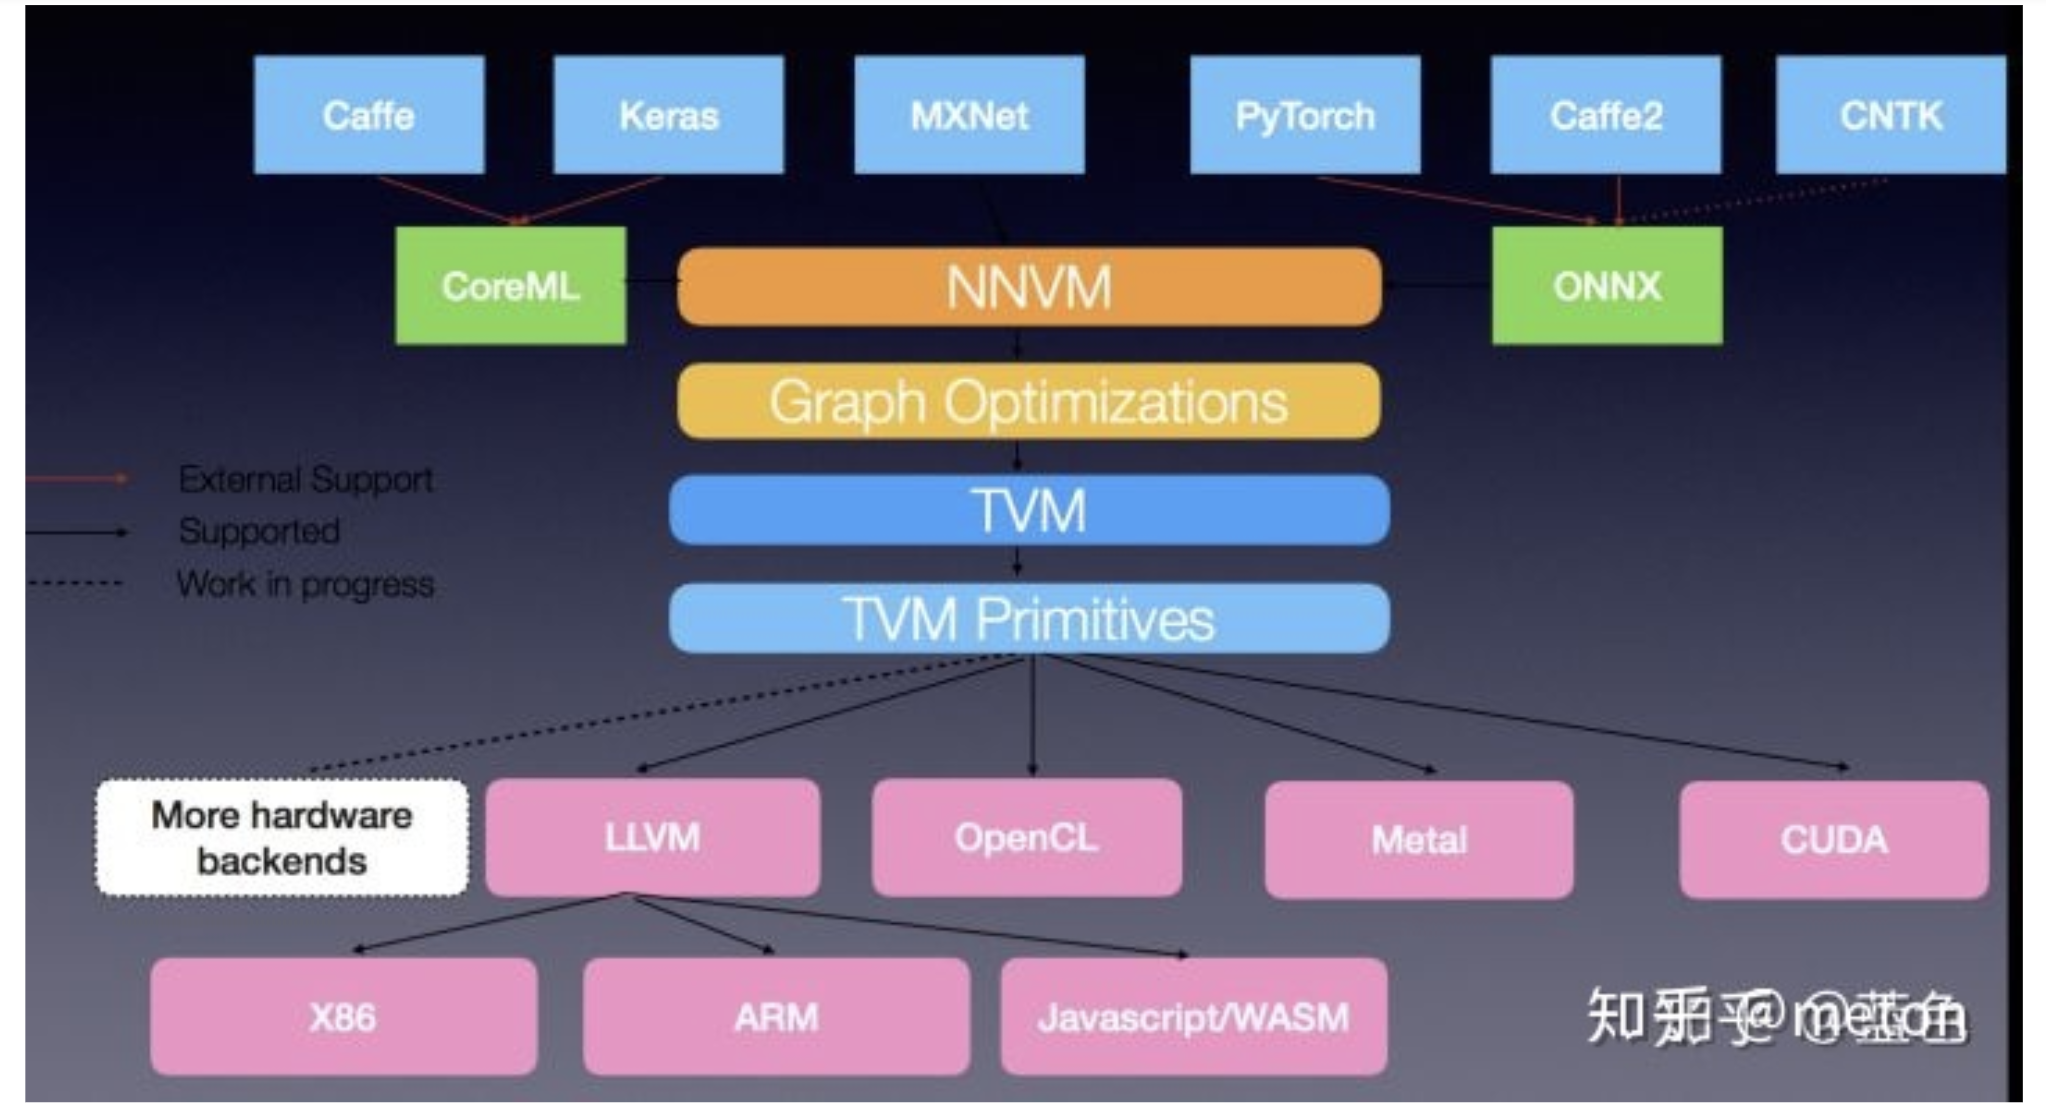
\includegraphics[width=1\textwidth]{fig/Deep_Learning_Speed_Up_TVM.png}
\end{figure}

从上图可以看出来,TVM其实是一个桥梁作用,TVM可以实现算子代码的自动生成,也就是说现在我在顶层训练好了模型需要部署到不同的目标平台,通过TVM可以生成针对这些平台的优化的算子和推理代码。当然自动生成的算子还可以结合手工进一步优化(自动与手工结合)。除了自动生成算子代码功能,TVM很有吸引力的一点就是其自动生成的代码可以媲美那些手工优化的加速库。

TVM的使用场景:
\begin{itemize}
\setlength{\itemsep}{0pt}
\setlength{\parsep}{0pt}
\setlength{\parskip}{0pt}
    \item 一种是离线支持敏捷算子优化,通过TVM自动代码生成的功能,部分解放优化人员手动添加优化的负担。具体地,给定一个计算,优化人员进行workload characterization分析完计算访存pattern之后,可以拟定几种可能的优化方案,如果TVM的schedule中包含,那么可以直接应用TVM来生成包含该优化的代码。然后借助profiler来分析代码的瓶颈,进一步修正或者更新优化方案,再试图借助TVM的自动生成能力,如此循环往复。到最后,如果TVM代码的可读性足够的话,优化人员可以在其上做手动优化;如果可读性不好的话,TVM也可以帮助优化人员快速确定优化方案。

    \item 另外一种场景是,运行时代码生成。当研究员在试验新的算子时,由于没有可供调用的计算库,同时缺乏CUDA等高性能代码开发经验,因此很多情况下是通过裸跑python代码来调用新算子的。PyTorch已经在今年5月份开始将TVM接入到PyTorch中实现运行时代码优化编译,目前已经可以运行了。
\end{itemize}
详细的讨论参考:《HONG:也谈TVM和深度学习编译器》\url{https://zhuanlan.zhihu.com/p/87664838} 和 《蓝色:手把手带你遨游TVM》 \url{https://zhuanlan.zhihu.com/p/50529704}

\subsection{Tensorflow XLA}
XLA(Accelerated Linear Algebra,加速线性代数)是一种优化TensorFlow计算的编译器。 XLA(加速线性代数)是为优化TensorFlow计算的特定领域编译器。它可以提高服务器和移动平台的速度、改进内存使用、提升便携性(或者说是可移植性)。 XLA框架是目前处于开发中的实验性项目。更多信息请阅读XLA指南,

XLA有几个与目标硬件无关的优化,例如公共子表达式消除(CSE,common subexpression elimination),过程与硬件后端无关的(target-independent)算子融合,以及用于为计算而在运行时做内存分配的缓冲区分析。

硬件目标无关的步骤之后,XLA将HLO计算发送到后端去做进一步的HLO级优化,HLO级优化会针对硬件目标特定信息和需求,如XLA GPU后端的算子融合、确定如何将计算划分为流。此阶段,后端还可以将某些算子或其组合与优化的库调用进行模式匹配。

下一步是特定于目标硬件的代码生成。CPU包括XLA使用的GPU后端会使用LLVM生成低级IR、优化和代码生成。硬件后端以有效方式发出了表示XLA HLO计算所必需的LLVM IR,然后调用LLVM从LLVM IR发出原生代码。
GPU后端目前通过LLVM NVPTX后端支持NVIDIA GPU,CPU后端支持多个CPU指令级架构( ISA)

详细可以参考:《按时计划:TensorFlow Lite概述:转换器、解释器、XLA和2019年路线图》\url{https://zhuanlan.zhihu.com/p/74085789}

\subsection{Pytorch Glow}
Glow是一个机器学习的编译器和执行引擎,它可以面向多种硬件, 是基于LLVM项目进行了开发的。

\section{体系结构与硬件设计}
传统标量处理器适合分支情况复杂的程序,但是对于深度学习这种数据驱动的、有明显的DLP特征的应用就显得不适用了,因此现在通常是通用处理器和专用处理器的结合,像我们手机有多个CPU负责一般程序执行,又有NPU去加速器一些神经网络应用。

\subsection{关注指标}
DNN加速器的关注的点不仅仅是 OPS/W,更多的是准确度、吞吐量、时延、功耗、硬件成本、硬件的灵活度或者说对新出现模型的可复用性等等各个方面的权衡。

\subsection{CPU与GPU平台}
现有的CPU和GPU都有官方的加速库来加速矩阵运算。CPU和GPU为了支持DLP行为,有专门的向量指令集,例如CPU的SIMD指令,不过SIMD毕竟是通用处理器对DLP的补充,并行度其实不算太高;还有就是GPU的SIMT,其实本质上是SIMD的一种不同的抽象方式,并且借助GPU大量的运算核心,在并行度方面远超支持向量处理的CPU。

SIMD和SIMT本质上是一种时间上的并行展开,属于Temporal架构,怎么理解呢?就好比一个循环并行,我每个并行计算单元做的是某次迭代的事,相当于把通用CPU在一段时间内的循环操作在我们的加速器的并行单元上一次性展开了。

进一步,有些CPU/GPU支持INT8 INT16低精度运算,在取相同的数据量情况下,还可以进行更多的乘法运算(4个INT8 相当于原先一个 FP32所占的空间)。

\subsubsection{CPU和GPU的设计考虑}
\textbf{软件(编译器)}

\begin{itemize}
\setlength{\itemsep}{0pt}
\setlength{\parsep}{0pt}
\setlength{\parskip}{0pt}
    \item 通过对卷积操作的变换来减少不必要的MACs,例如前面提到的卷积近似计算
    \item 通过编译时的优化PASS对循环执行进行调度(循环展开、循环tile等等)
    \item 编译器优化减少load,store指令,尽量用寄存器操作
\end{itemize}

\textbf{硬件}

\begin{itemize}
\setlength{\itemsep}{0pt}
\setlength{\parsep}{0pt}
\setlength{\parskip}{0pt}
    \item 提高PEs处理每个MAC的时间
    \item 提高并行度(使用更多并行的PEs,例如PE阵列)
    \item 提高PE的利用率. 意思是尽量使得PE忙碌,一个方法是增加片上缓存大小,提高访存总线宽度等等入手,这些都旨在减少访存的瓶颈,PEs可以更快拿到数,减少等待时间;另一种方式是让数据尽可能在数据通路中多停留,这样在访存能力不变的情况下,就可以用流水线的形式让PE尽可能有事做,后面讲解的TPU所用的脉动阵列,和流行的 DtaFlow数据流架构都是类似方式,当然在GPU的设计上也可以融入上述通用思想
\end{itemize}

\subsection{Domain-Specific 硬件设计}
\subsubsection{设计关注点}
DNN加速器在体系结构设计所关注的几个点:数据的读写也就是访存,以及计算。尤其是访存问题,因为通常PE数目很容易堆上去,并行度上去后,数据读写往往会成为瓶颈,也就是常说的撞到“内存墙”,内存访问在我们的机器上是有层级的,寄存器,cache很快,但是到了内存取数就很慢,数据在cache miss后代价会很大,因此如果没有很好的访存优化,那么对于大数据的深度学习,加速比是很难做上去的。

从DNN加速器的经典实现 DianNao系列、TPU、Eyeriss来看(后面会讲到),这些加速器都十分关注访存方面的设计,后续有时间就其一些设计细节展开。不过大体上优化访存的方式有:
\begin{itemize}
\setlength{\itemsep}{0pt}
\setlength{\parsep}{0pt}
\setlength{\parskip}{0pt}
    \item 研究新的内存制作工艺:这个没那么没那么容易其实
    \item 从更下级cache取数:一般CPU从L1 cache取数,但是L1 cache能装的数比较少,我看到有些加速器从L2 cache取数,因为L2 更大一些,取数 miss几率小,不过这么做要解决一下cache一致性问题(Hwacha)
    \item 增大加速器的片上buffer:好理解,如果我加速器的buffer大的可以装进更多权重,那么计算部件PE要消费数据的时候取数从片上buffer取,那肯定比从内存取数要快
    \item 数据重用:如果这个PE产生的结果下一次计算会被接着用上,那么可以让这个数据留在PE中,等待下次复用,这样就减少了数据被store回去、下一次又load回来的开销。从另外一个角度看,第二种方式本质上也是在利用数据的复用,只不过把数放在片上buffer来复用,复用的粒度不同
\end{itemize}

两类设计范式:
\begin{itemize}
\setlength{\itemsep}{0pt}
\setlength{\parsep}{0pt}
\setlength{\parskip}{0pt}
    \item Temporal Arch. 这个前面有提及主要以SIMD,SIMT为代表
    \item Spatial Arch. 也就是数据流模式. 相比Temporal Arch的不同之处就是,数据流模式中PE与PE之间是可以相互通信的,也就是说数据可以在PE间流动,这一周期计算出来的结果可以在下一周期流到其他PE参与运算,而不用发生访存动作。所以,这样带来的好处是有更大的数据吞吐量,适合具有很好数据重用特性的应用
\end{itemize}

\subsubsection{深度学习应用的data reuse机会}
前面说道,处理访存问题是DNN加速器设计的一个关键,一个方法就是发掘卷积操作中的数据复用性。

卷积神经网络三个角度复用,一是复用权重;二是复用激活(也就是feature map);三是复用两者。不同的复用策略,可以引申出不同设计架构和取数策略。



%\printbibliography
\bibliography{../ref}
\bibliographystyle{IEEEtran}
\end{document}
